\documentclass{article}%You can define the type of paper here.
%%Useful packages that I commonly use.
\usepackage[numbers]{natbib}%Bibliography package (help at http://merkel.zoneo.net/Latex/natbib.php).
\usepackage{url}%Package to highlight url.
\usepackage{times}%Sets font to be times.
\usepackage{alltt}%Allows the use of verbatim (good for printing out code).
\usepackage{graphicx}%Used to import images.
\usepackage{amsmath, amssymb, amscd, gensymb}%Contains the AMS expanded math symbols library.
\usepackage{upgreek}
%%For those who want smaller margins, you can use this:
\usepackage[top=1in, bottom=1in, left=1in, right=1in]{geometry}

\begin{document}

    %%Title
    \title{Simulation and Modeling\\Final Project: Simulating Traffic Flow with Cellular Automata}
    \author{Clinton McKay}
    \maketitle

    %%Makes the paper use two collums
    \twocolumn

    %%Introduction-------------------------------------------------------------------------------------
    \section{Introduction}
    The first know description of cellular automation was by Von Neumann. 
    His goal was figure out the components required to implement a machine that could self replicate.  
    Another well know program that uses cellular automata would be Conway's Game of Life which can result in complex patterns and can be used to simulate a simple processors. 
    At first, it would appear that CA (cellular automation) techniques are nothing more than an oddity for academic interest. Instead the it has been proven that cellular automation is quite effective in modeling several problems. For example traffic flow on a single lane freeway \cite{nagel:freeway}  and a dual lane freeway \cite{rickert:twolane}, and crowd flows \cite{zhen:crowd-evac}, \cite{zhao:crowd-evac}, and \cite{kats:crowd-flow}. 
    For this project I have decided to model the speed at which pedestrians can evacuate a room based on their movement parameters and the number of available exits. 

    %%Method------------------------------------------------------------------------------------------
    \section{Method}
    Upon further investigation into simulating traffic flow with cellular automata. The differences between the algorithms are large enough that they have inherited a separate discussion each. First we will focus on the original CA algorithm for traffic flow which was introduced in the 1990's by Kai Nagel \cite{nagel:freeway}. Followed by an extension of that algorithm to account for multilane traffic. Afterwards we will discuss an algorithm that was used to simulate the flow of ants and pedestrians \cite{kats:crowd-flow}. 

    \subsection{ Freeway Traffic }

    In 1992 Kai Nagel proposed a computation model that takes a single dimensional array $W$ with $L$ sites that has periodic boundaries \cite{nagel:freeway}. Each site in $W$ represents a location that may have a vehicle in it. Since the system is discrete all vehicles that belong to $W$ may only have a positive integer velocity. Updates to the system must follow a four step procedure \cite{nagel:freeway}.

    \begin{enumerate}
        \item {\bf Acceleration:} If the velocity $v$ of a vehicle is less than the speed limit $v_max$ and if the distance to the next car ahead is larger than $v + 1$ then increment the velocity by one. 
        \item {\bf Slowing down (for other cars):} If there exists a vehicle $v_{j+n}$ in front of another vehicle $v_j$ then $v_j$ must decrease it's speed to $v = n - 1$ (the size of the gap between the two vehicles). 
        \item {\bf Randomization:} Humans drive sporadically apply a random fluctuations to the velocity. Nagel's implementation only applies random accelerations. My algorithm was slightly modified so that random decelerations can accounted for. 
        \item {\bf Move:} Update the vehicle positions based on their velocity. 
    \end{enumerate}

    The implementation of this algorithm can be observed in {\it TrafficFlowSingleLane-CellAut.nlogo} within the {\it \bf update} function. 
    
    \subsubsection{ Freeway Traffic Two-lane}

    To further investigate traffic flow, M. Rickert's modification of the algorithm \cite{rickert:twolane} was implemented. The algorithm isn't much different except that has been split into two sub-steps. The new rules are:

    \begin{enumerate}
        \item Check the left and right lanes for larger gaps. If a larger gap is found jump with probability $p$ to the appropriate lane. The vehicle will only move to a different lane. Its position $l$ in $L$ will not change. Velocity changes are accounted for in step 2.  
        \item Perform the Nagel's algorithm.
    \end{enumerate} 

    This algorithm allows vehicles to flow at higher rates than the first algorithm where vehicles are more dependent of the velocity in front of them. An implementation of this algorithm can be found in the {\bf update} function inside of {\it TrafficFlowTwoLanes-CellAut.nlogo}. 

    \subsection{ Pedestrian Flow }
    The flow of traffic is an interesting phenomenon, but it can be limited in scope since vehicle motion is bound to the rules of the road. A more interesting model is one that provides greater importance to the freedom of the particles moving in the system. Such models allow the simulation of pedestrians or other biological life forms. For this project, I decided to implement a model by Nishinari \cite{kats:crowd-flow}.  

    \begin{enumerate}
        \item The dynamic floor $D$ is modified according to its diffusion and decay rules. 
        \item For each pedestrian, construct a set of weights $p_{ij}$ that can be used to select potential future positions. The formula is:
        \begin{align*}
            p_{ij} = e^{k_DD_{ij}}e^{k_SS_{ij}}P_I(i, j) * \upxi_{ij} 
        \end{align*}
        $D_{ij}$ represents the pheromones at each site in the world. Since this is a simulation of an evacuation then the pheromones represent the adrenaline released into the air. Other pedestrians are attracted to this. $k_D$ represents the panic factor, the higher a value of $k_D$ the more random the movements of the pedestrians become. 

        $k_S$ and $S_{ij}$ represent the distance and weight to the goal site. Relative to my implementation, $k_S$ is the inverse diffused height between the source and sink on the map, while $S_{ij}$ has been set to a constant of one for all sites. 

        $P_I$ represents the inertial of the pedestrian. It is affected by their heading. Given the scope of this project $P_I$ is a constant. 
        \item After constructing the weights, use them to sample the next location of the pedestrian. Move to that location. 
        \item After moving the pedestrians. Backtrack pedestrians that have landed on the same site to their old positions. Sample a pedestrian to stay at the new location.
\end{enumerate}

    %%Verification------------------------------------------------------------------------------------
    \section{Verification of Program}      
    The algorithms where implemented using NetLogo an agent based programming language. The NetLogo application is designed such that the programmer can construct prototypes quickly by allow the creation of an interface, integration of documentation as markdown, and an area to write code for more advanced logic.

    There are three NetLogo applications. {\it TrafficFlowSingleLane-CellAut.nlogo, TrafficFlowTwoLanes-CellAuto.nlogo} and {\it CrowdFlow.nlogo}. The first file contains the necessary components to implement the single lane lane algorithm. The second file contains the traffic simulation with agents that can change lanes based on the gap size ahead. 
    
    The third file (and the most complex) implements the pedestrian flow algorithms, allows you to setup your own scenarios, save and export them. 

    Descriptions on how to use the programs are detailed in the {\it info} section of the nlogo files. 


    %%Data--------------------------------------------------------------------------------------------
    \section{Data}
    \subsection{ Traffic Simulations }
    $p_b$, $p_a$, and $p_l$ represent the breaking probability, acceleration probability, and lane change probability respectively.
    
    \begin{figure}[ht!]
        \centering
        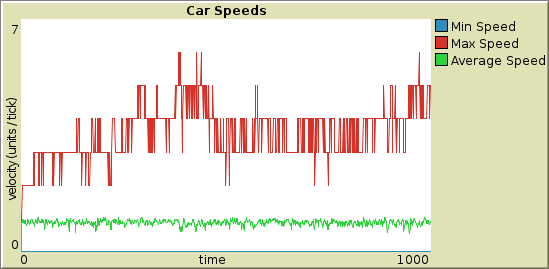
\includegraphics[width=3in]{../img/VelocitiesSingleLane.png}
        \caption{Single lane simulation: 31 cars with initial uniform placement and velocity of zero. $p_b = 0.10$, $p_a = 0.20$, and $v_{max} = 6$}
        \label{vsl:31:0d1:0d2}
    \end{figure}
    
    \begin{figure}[ht!]
        \centering
        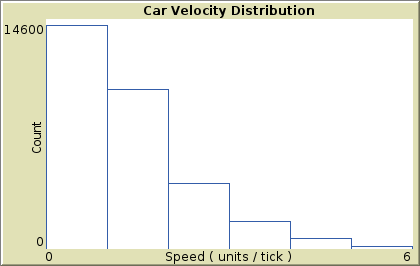
\includegraphics[width=3in]{../img/VelDistroSingleLane.png}
        \caption{Single lane simulation: Distribution with same parameters as Figure \ref{vsl:31:0d1:0d2}}
        \label{vsl:d31:0d1:0d2}
    \end{figure}

    Disabling the random acceleration behaviors results in a more unrealistic and predictable system. 

    \begin{figure}[ht!]
        \centering
        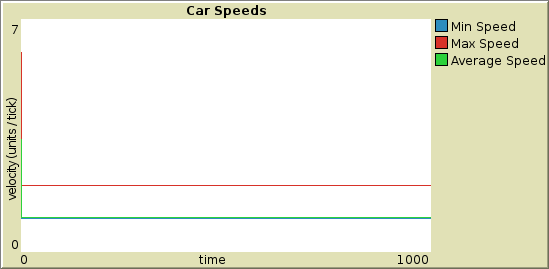
\includegraphics[width=3in]{../img/VelocitiesSingleLane_pb0pa0.png}
        \caption{Same initial conditions as Figure \ref{vsl:31:0d1:0d2} except $p_b = 0$ and $p_a = 0$.}
        \label{vsl:31:0d0:0d0}
    \end{figure}
 
    \begin{figure}[ht!]
        \centering
        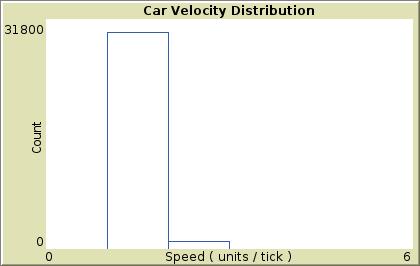
\includegraphics[width=3in]{../img/VelDistroSingleLane_pb0pa0.png}
        \caption{Speed distributions for Figure \ref{vsl:31:0d0:0d0}}
        \label{vsl:d31:0d0:0d0}
    \end{figure}

    \begin{figure}[ht!]
        \centering
        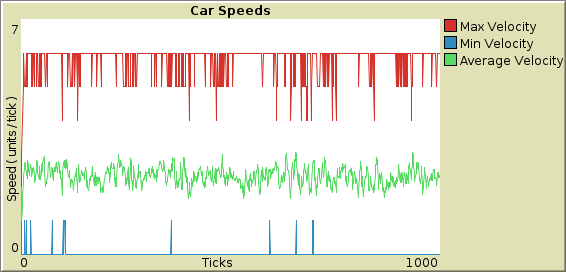
\includegraphics[width=3in]{../img/VelocitiesTwoLane.png}
        \caption{Dual lane simulation: 30 cars with initial uniform placement and velocity of zero. $p_b = 0.10$, $p_a = 0.20$, $p_l = 0.30$, and $v_{max} = 6$}
        \label{vtl:31:0d1:0d2}
    \end{figure}
    
    \begin{figure}[ht!]
        \centering
        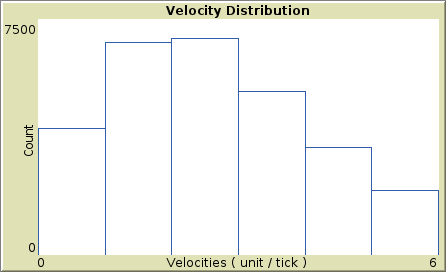
\includegraphics[width=3in]{../img/VelDistroTwoLane.png}
        \caption{Dual lane simulation: Distribution with same parameters as Figure \ref{vtl:31:0d1:0d2}}
        \label{vtl:d31:0d1:0d2}
    \end{figure}

    After disabling the random fluctuations for the dual lane traffic simulation. 

    \begin{figure}[ht!]
        \centering
        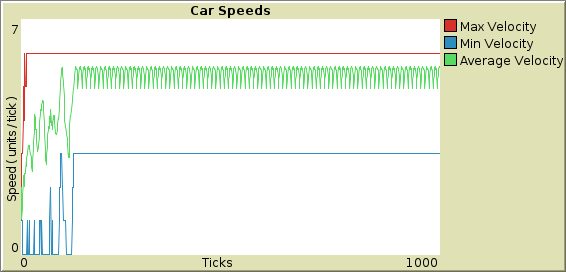
\includegraphics[width=3in]{../img/VelocitiesTwoLane_pb0pa0.png}
        \caption{Dual lane simulation: Distribution with initial conditions as Figure \ref{vtl:31:0d1:0d2}, except $p_b = 0$ and $p_a = 0$}
        \label{vtl:31:0d0:0d0}
    \end{figure}

    \begin{figure}[ht!]
        \centering
        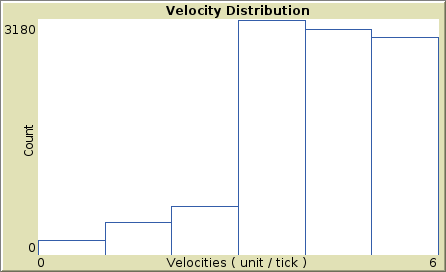
\includegraphics[width=3in]{../img/VelDistroTwoLane_pb0pa0.png}
        \caption{Velocity distribution from Figure \ref{vtl:31:0d0:0d0}}
        \label{vtl:d31:0d0:0d0}
    \end{figure}

    \subsection{ Crowd Flow }
    Results from the crowd flow simulations. Since the crowd flow algorithm wasn't working properly the plots produced are not an accurate representation of how the algorithm should behave. All of the plots represent the flux (the average number of people who left per tick) and the population density of the room. In this case the room chosen has a width of 34 and height of 54 units. Figures 9 through 15 visualize the flux and change of density over time as a function of the crowd panic and the starting density of the room. The panic level and pheromone decay probability are denoted as $p_l$ and $p_d$. All doors are assumed to have size of one such that only a single person can pass through the doorway. 

    \begin{figure}[ht!]
        \centering
        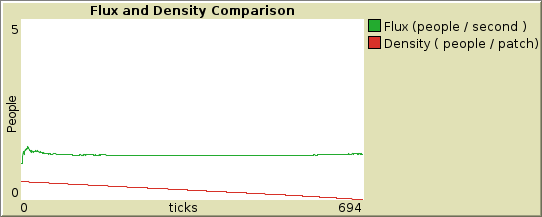
\includegraphics[width=3in]{../img/Crowd34x541d_pl0pd0d5.png}
        \caption{ Observation of flux and density change given a starting room population of 875 out of a maximum capacity of 1750 with $p_l = 0$ and $p_d = 0.5$. Given the room has a single door.}
        \label{crd:d1:pl0:pd0d5}
    \end{figure}

    \begin{figure}[ht!]
        \centering
        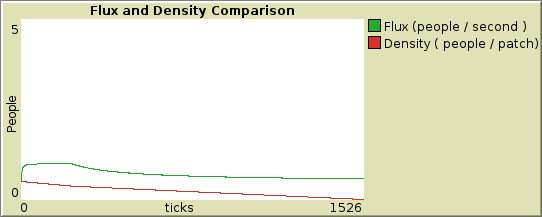
\includegraphics[width=3in]{../img/Crowd34x541d_pl10pd0d5.png}
        \caption{ Same conditions as Figure \ref{crd:d1:pl0:pd0d5} except $p_l = 10$.}
        \label{crd:d1:pl0:pd0d5}
    \end{figure}

    \begin{figure}[ht!]
        \centering
        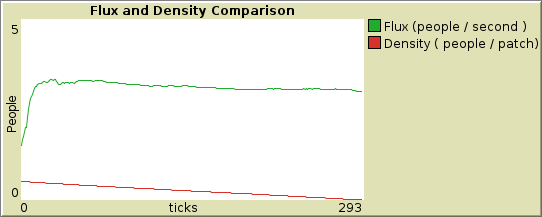
\includegraphics[width=3in]{../img/Crowd34x542d_pl0pd0d5.png}
        \caption{The flux and density change of a room that has two doors. The starting population is 875 out of a maximum capacity of 1750 with $p_l = 0$ and $p_d = 0.5$}
        \label{crd:d2:pl0:pd0d5}
    \end{figure}

    \begin{figure}[ht!]
        \centering
        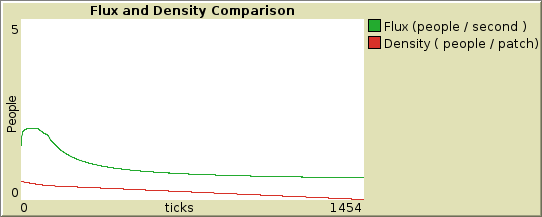
\includegraphics[width=3in]{../img/Crowd34x542d_pl10pd0d5.png}
        \caption{Same initial settings as Figure \ref{crd:d2:pl0:pd05} except $p_l = 10$}
        \label{crd:d2:pl10:pd0d5}
    \end{figure}

    \begin{figure}[ht!]
        \centering
        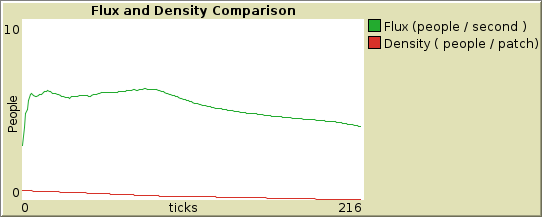
\includegraphics[width=3in]{../img/Crowd34x544d_pl0pd0d5.png}
        \caption{ Observation of flux and density change given a starting room population of 875 out of a maximum capacity of 1750 with $p_l = 0$ and $p_d = 0.5$}
        \label{crd:d4:pl0:pd0d5}
    \end{figure}

    \begin{figure}[ht!]
        \centering
        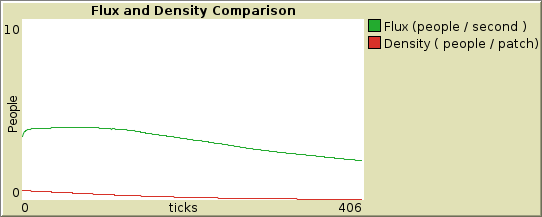
\includegraphics[width=3in]{../img/Crowd34x544d_pl10pd0d5.png}
        \caption{Same as Figure \ref{crd:d4:pl0:pd0d5} except $p_l = 10$}
        \label{crd:d4:pl10:pd0d5}
    \end{figure}
    
    %%Analysis---------------------------------------------------------------------------
    \section{ Analysis }

    When the random fluctuations in speed are removed from the vehicles ($p_b = p_a = 0$). Then the average velocity appears to increase dramatically. Increasing the fluctuation rate a causes the average velocity to decrease for the vehicles. By adding an extra lane the vehicles are able to compensate for the fluctuation and keep a higher average velocity. 

    Even though the crowd simulation algorithm didn't work properly. Some interesting properties became visible. When the randomness of the crowd motion increased so did the flux, but if the randomness of the crowd motion decreased the flux value also decreased.    

    %%Interpretation---------------------------------------------------------------------
    \section{ Interpretation }

    The implementation of the traffic simulation worked quite well and it turned out easier then I originally expected. It would be interesting to implement more complex road structures and observe how the motions of the vehicles differ when there are multiple intersections. 

    Besides the traffic simulations, further investigation of the crowd flow algorithm would be needed in order to figure out the strange behavior of the panic level. Instead of increasing the random motion of the people instead it decreases it. 

    %%Bibliography-----------------------------------------------------------------------
    \nocite{*}
    \bibliography{sources}
    \bibliographystyle{acm}

\end{document}
